\documentclass[aspectratio=169]{beamer}
\usetheme{default}
\usecolortheme{dove}
\setbeamertemplate{navigation symbols}{}
\setbeamerfont{title}{size=\Large}
\setbeamerfont{frametitle}{size=\large}

\usepackage{fontenc}
\usepackage{inputenc}
\usepackage[danish,english]{babel}
\usepackage{graphicx}
\usepackage{booktabs}

\title{Ludvig Holberg (1684--1754)}
\subtitle{Setting the Stage}
\date{PHI 423 \textbar{} The Modern Breakthrough in Scandinavia}

\begin{document}

\begin{frame}
  \titlepage
\end{frame}

%% --- Who was he? ---

\begin{frame}{A man between two worlds}
  \begin{columns}
    \begin{column}{0.65\textwidth}
      \begin{itemize}
        \item Born Bergen, Norway (1684); died Copenhagen (1754)
        \item Spent his career at the University of Copenhagen
          --- professor of metaphysics, then rhetoric, then history
        \item A European intellectual: Oxford, Paris, Rome, Hamburg
        \item Founder of modern Danish-Norwegian literature and theatre
        \item \emph{Also} a systematic moral and political philosopher
      \end{itemize}
    \end{column}
    \begin{column}{0.32\textwidth}
      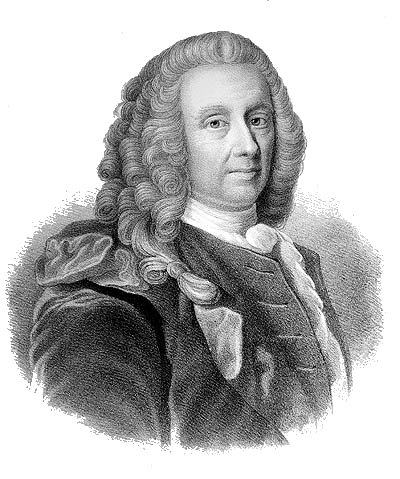
\includegraphics[width=\textwidth]{resources/holberg.jpg}
    \end{column}
  \end{columns}
\end{frame}

%% --- What did he write? ---

\begin{frame}{The philosophical work}
  \begin{description}
    \item[\normalfont\textit{Introduction til Naturens og Folke-Rettens Kundskab}
      (1716)] Natural law freed from theology; required reading for Danish law
      students until 1936
    \item[\normalfont\textit{Moralske Tanker} (1744)] 63 Montaigne-style essays ---
      ironic, paradoxical, anti-dogmatic
    \item[\normalfont\textit{Epistler} (1748--54)] Philosophy in a conversational
      register; four volumes
    \item[\normalfont\textit{Niels Klim} (1741)] Utopian satire --- European customs
      defamiliarised from underground
  \end{description}
\end{frame}

%% --- Where does he stand? ---

\begin{frame}{Holberg's intellectual position}
  \begin{itemize}
    \item \textbf{Empiricist}: knowledge grounded in experience; follows Locke and
      the English tradition he absorbed at Oxford
    \item \textbf{Anti-systematic}: eclectic by principle, suspicious of grand
      metaphysical architectures
    \item \textbf{Natural law moralist}: ethics grounded in reason and social
      utility, not revealed religion
    \item \textbf{Deist}: critical of pietism and revealed theology, but not
      irreligious
  \end{itemize}
\end{frame}

%% --- Høffding's Danske Filosoffer ---

\begin{frame}{Holberg in the Danish philosophical tradition}
  \begin{columns}
    \begin{column}{0.55\textwidth}
      Harald H\o ffding's \textit{Danske Filosoffer} (1909) surveys the
      history of philosophy in Denmark and Norway.

      \medskip
      Holberg is \textbf{Chapter~1} --- the founding figure from whom
      the whole tradition flows.
    \end{column}
    \begin{column}{0.42\textwidth}
      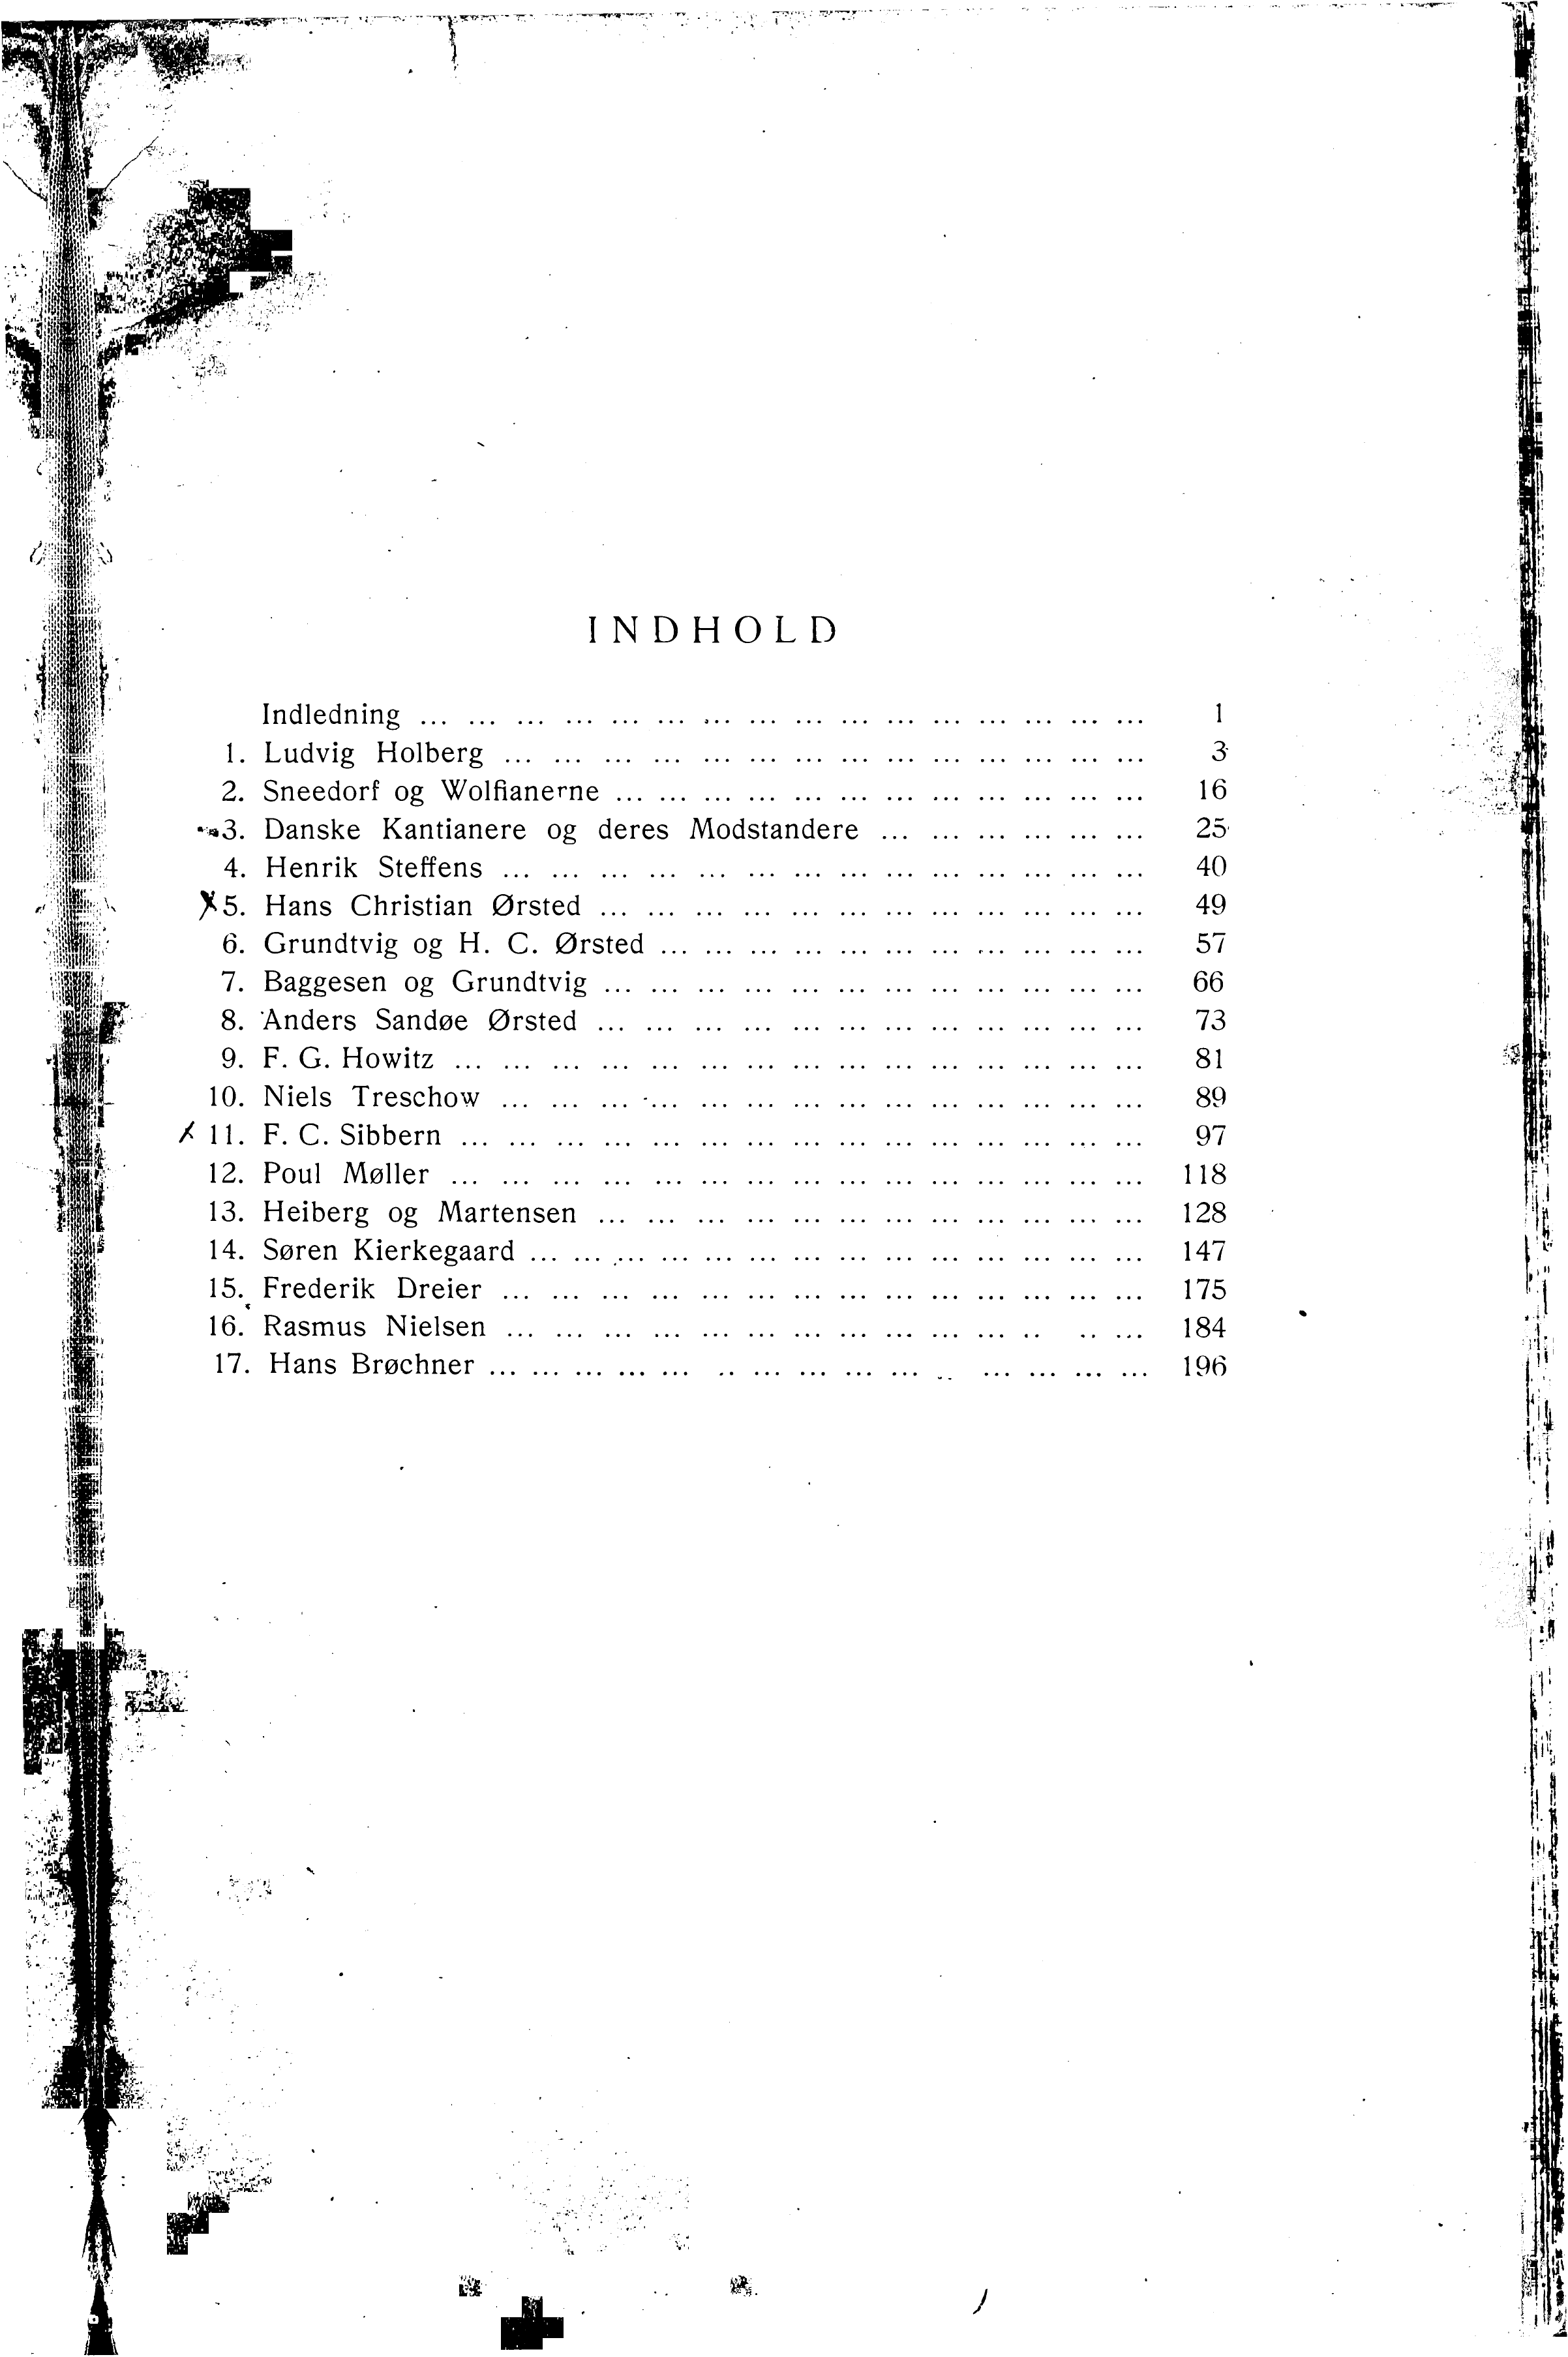
\includegraphics[width=\textwidth]{resources/hoffding-toc.png}
    \end{column}
  \end{columns}
\end{frame}

%% --- Why does he matter for this course? ---

\begin{frame}{Why Holberg matters for this course}
  \textbf{He sets the tone for the tradition we are studying.}

  \medskip
  \begin{itemize}
    \item H\o ffding calls him the first Danish philosopher to engage \emph{independently}
      with the problems of thought --- ``\foreignlanguage{danish}{den første herhjemme,
      der på selvstændig måde tager stilling til tankens problemer}''
    \item Aall: Holberg is the founder of
      \emph{\foreignlanguage{danish}{den dansk-norske individualisme}} ---
      resistance to German system-philosophy, insistence on experience
    \item Allen: Holberg is Kierkegaard's unacknowledged mentor --- irony,
      indirect communication, the ridicule of pedantry and crowd-conformism
  \end{itemize}
\end{frame}

%% --- The comedies ---

\begin{frame}{\textit{Erasmus Montanus} (1723)}
  \begin{columns}
    \begin{column}{0.65\textwidth}
      The paradigm case of Holbergian satire:

      \medskip
      \begin{itemize}
        \item Rasmus Berg returns from Copenhagen as ``Erasmus Montanus''
        \item Armed with syllogisms, he proves the earth is round --- and that his
          mother is a stone
        \item The village sees him as arrogant and dangerous; he recants to marry
          and be left in peace
      \end{itemize}

      \medskip
      \textit{What is Holberg satirising --- the pedant, or the crowd?
        Or both?}
    \end{column}
    \begin{column}{0.32\textwidth}
      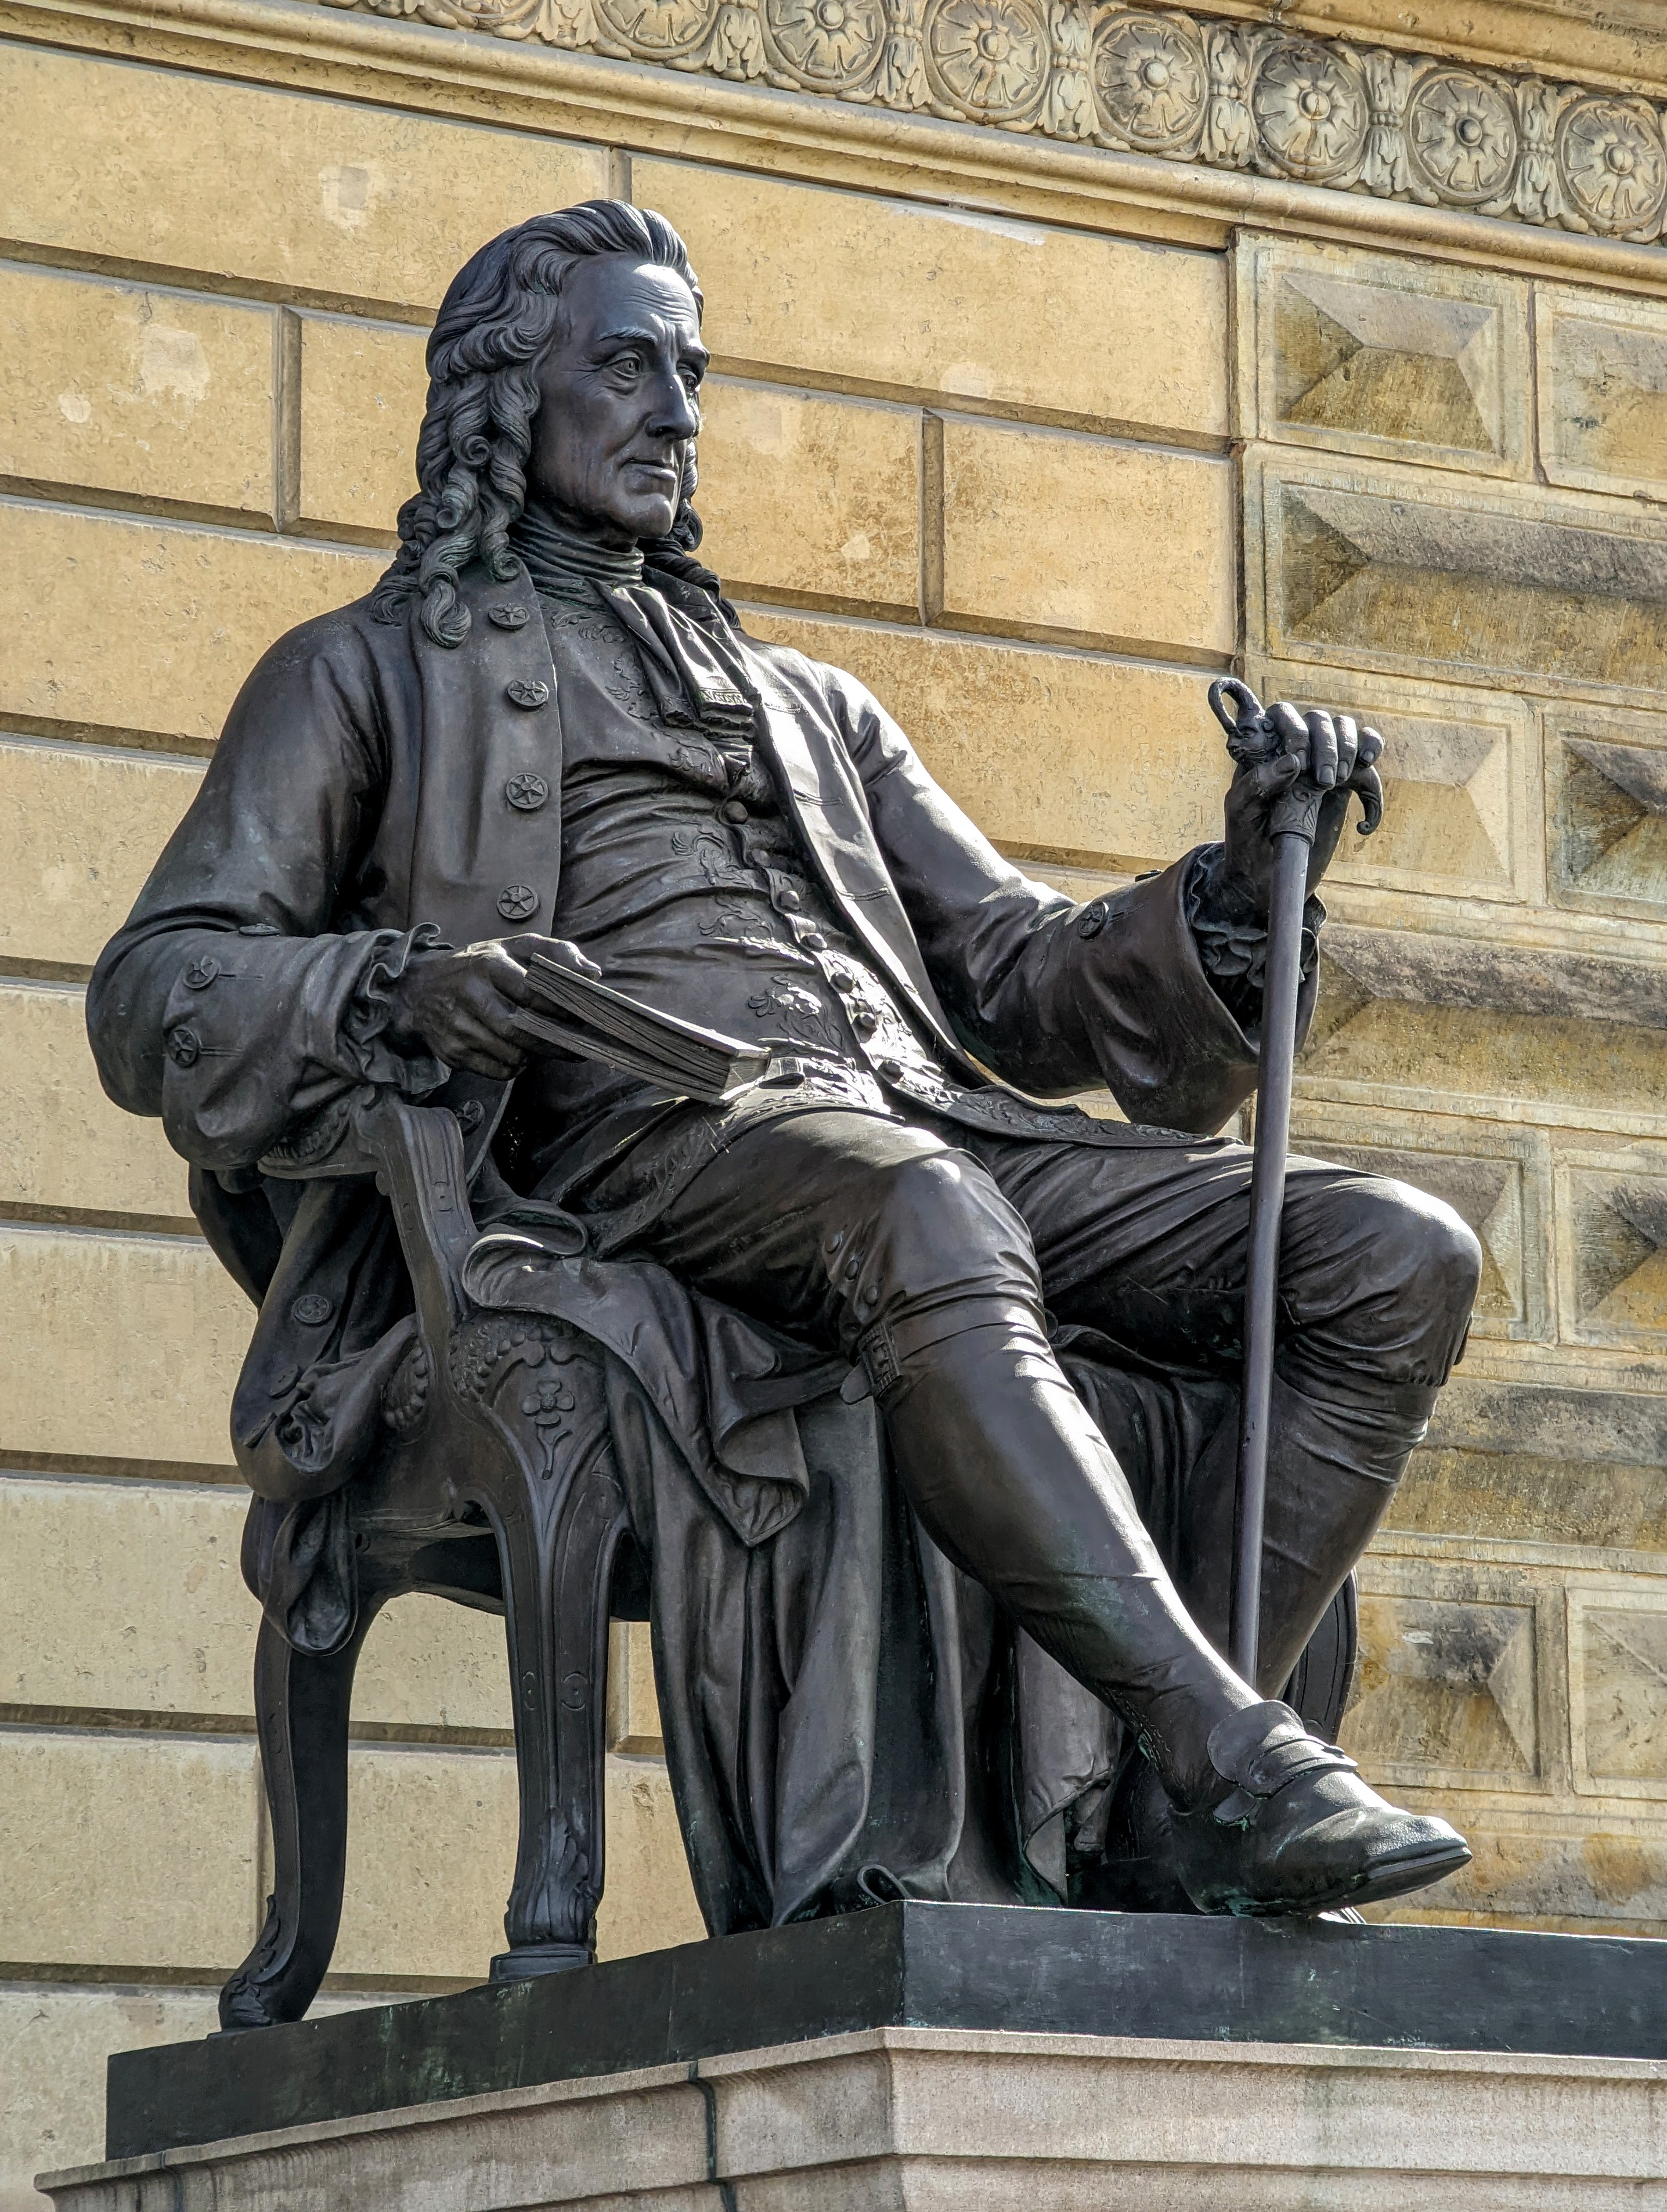
\includegraphics[width=\textwidth]{resources/holberg2.jpg}
    \end{column}
  \end{columns}
\end{frame}

%% --- Take-away ---

\begin{frame}{The thread to follow}
  \begin{center}
    \large
    Holberg establishes a philosophical style: \\[6pt]
    concrete, ironic, anti-systematic, morally serious.

    \bigskip
    \normalsize
    This style --- not any specific doctrine --- is what gets transmitted\\
    to Kierkegaard, Brandes, and the Modern Breakthrough writers.
  \end{center}
\end{frame}

\end{document}

%%% Local Variables:
%%% mode: latex
%%% TeX-master: t
%%% End:
